\section{Experiments}

Initial experiments involved using the entire LSTM output sequence as input to the FC layer. This approach resulted in unusable predictions, with the model often producing unrealistic price jumps between consecutive predictions. Adjusting the loss function, model size, and other hyperparameters did not resolve this issue. Switching from using the entire LSTM output to the last single LSTM output led to more stable predictions. 

\begin{figure}[h]
    \centering
    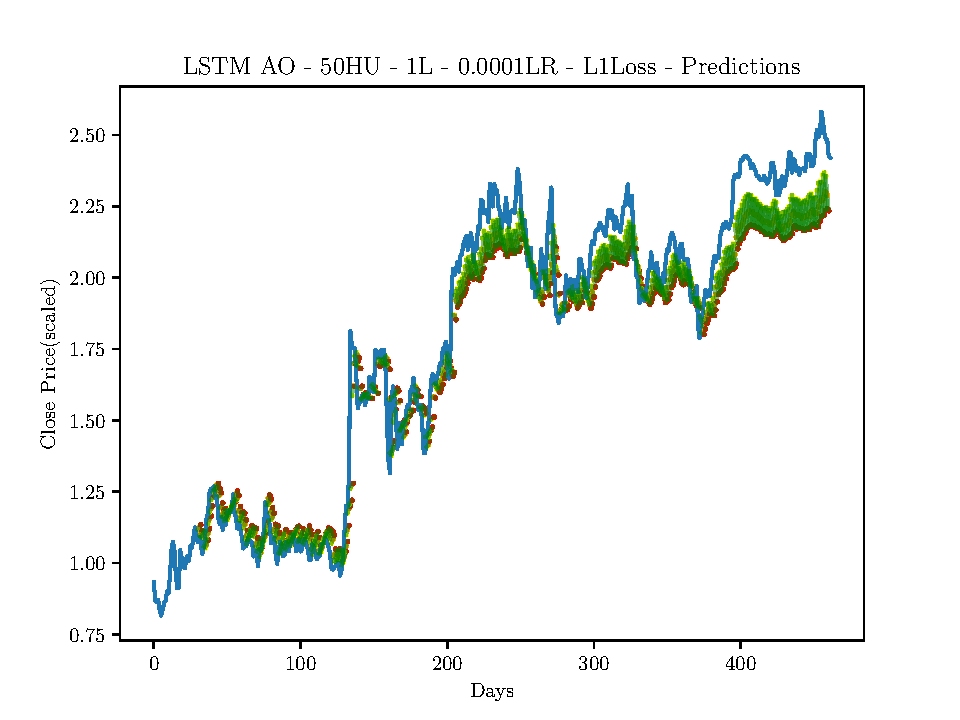
\includegraphics[width=0.5\textwidth, trim=20 0 20 10, clip]{plots/LSTM AO - 50HU - 1L - 0.0001LR - L1Loss-predictions.pdf}
    \caption{Predictions of the model with 50 hidden units and 1 layer. Green lines represent the predictions, red markers indicate the 3 predicted day.}
    \label{fig:ao_50HU_1L}
\end{figure}

\begin{figure}[h]
    \centering
    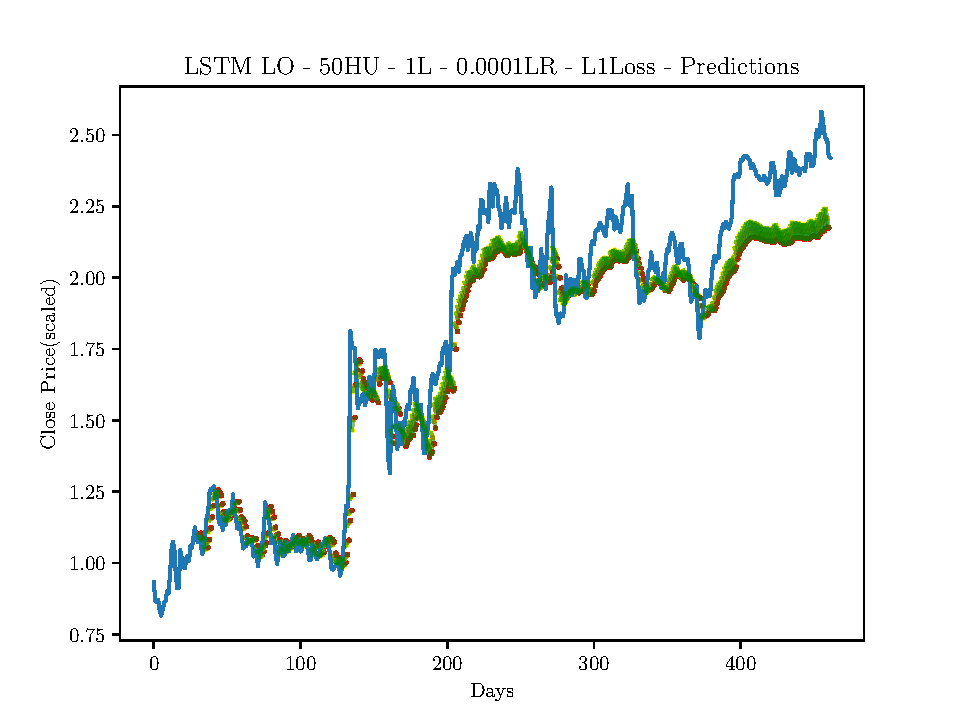
\includegraphics[width=0.5\textwidth, trim=20 0 20 10, clip]{plots/LSTM LO - 50HU - 1L - 0.0001LR - L1Loss-predictions.pdf}
    \caption{Predictions of the model with 50 hidden units and 1 layer. Green lines represent the predictions, red markers indicate the 3 predicted day.}
    \label{fig:lo_50HU_1L}
\end{figure}


The experiments started with the following hyperparameters: 5 input features, 5 output features, 50 hidden units, 1 layer, L1 loss, 0.0001 learning rate(LR), 1e-5 weight decay. Both model varients for 50 hidden units can be viewed in Figure \ref{fig:ao_50HU_1L} and Figure \ref{fig:lo_50HU_1L}.

\begin{figure}[h]
    \centering
    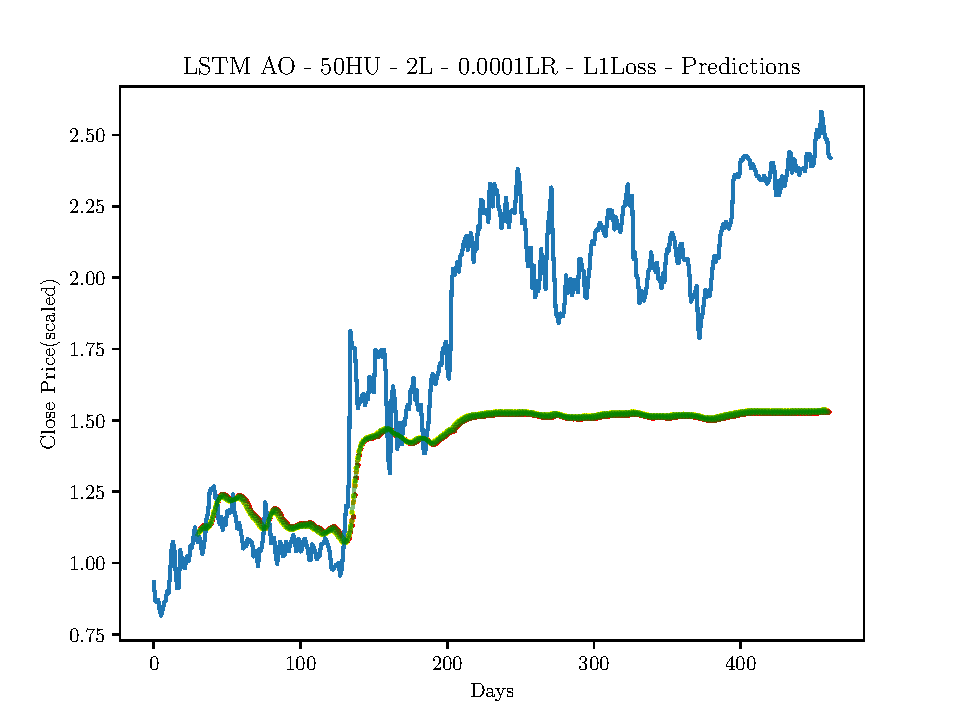
\includegraphics[width=0.5\textwidth, trim=20 0 20 10, clip]{plots/LSTM AO - 50HU - 2L - 0.0001LR - L1Loss-predictions.pdf}
    \caption{Predictions of the model with 50 hidden units and 2 layers. Green lines represent the predictions, red markers indicate the 3 predicted day. The predictions are smoothed out too much and resemble a moving average.}
    \label{fig:smoothed_out}
\end{figure}

Using 2 or more layers resulted in the predictions being smoothed out too much, see Figure \ref{fig:smoothed_out}, and resembles a moving average. This also caused no buys to be made with the strategy as time progressed since the Google stock price increases over time. The quality of the predictions do not look good as once the price gets high, the model always predicts the price to decrease.

As can be seen in Table \ref{tab:results}, 20 hidden units has a higher loss but performs well with the strategy. 50 and 100 hidden units have a lower loss but perform worse with the strategy. This is likely due to the model overfitting to the training data.

L1Loss seems to be important for the model to perform well. In Table \ref{tab:results}, L1Loss performed the best for the LSTM using the last output, while SmoothL1Loss(which is L1Loss \& MSELoss) performed the best for the LSTM using the entire output. MSELoss performed the worst in all cases. Note we can not compare the loss values directly between the different loss functions as they are calculated differently.

All the model variations converged well during training with a smooth loss curve, see Figure \ref{fig:loss_curve}. But it can also be seen that the model is heavily overfitting to the training data. Weight decay alone was not enough to prevent this.

\begin{figure}[h]
    \centering
    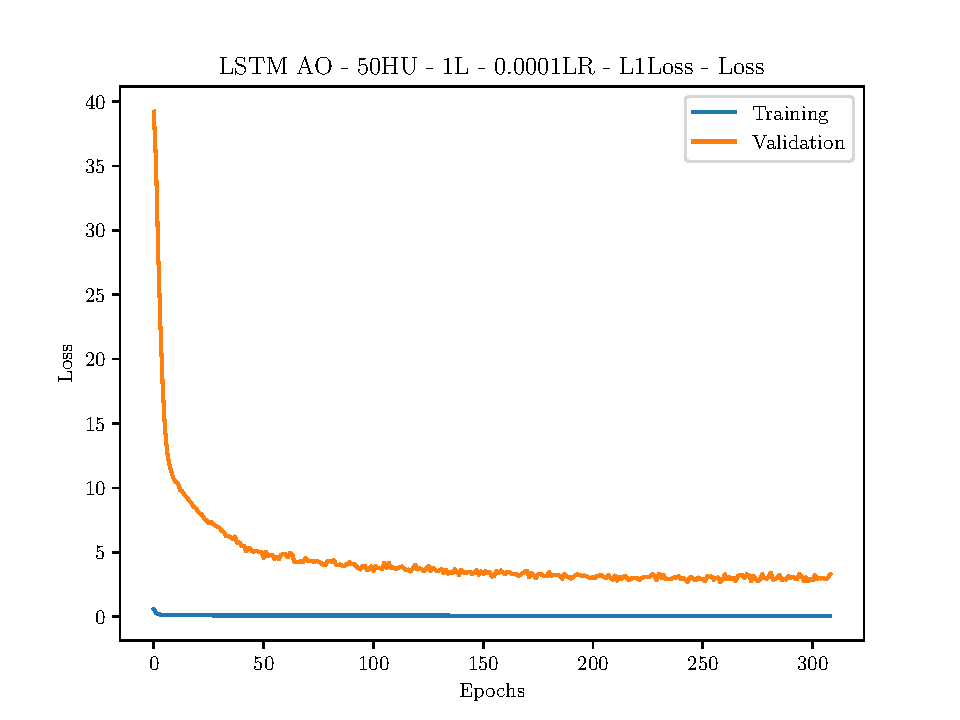
\includegraphics[width=0.5\textwidth, trim=20 0 20 10, clip]{plots/LSTM AO - 50HU - 1L - 0.0001LR - L1Loss-loss.pdf}
    \caption{Loss curve of the model with 50 hidden units and 1 layer.}
    \label{fig:loss_curve}
\end{figure}

\begin{table}[h]
    \centering
    \begin{tabular}{lcc}
        \hline
        \textbf{Model} & \textbf{Val. Loss} & \textbf{Return(\%)} \\ \hline
        w/all 100HU & 2.71 & 57 \\ 
        w/all 50HU & 2.66 & 71 \\ 
        w/all 20HU & 3.63 & 89 \\
        \hline
        w/last 100HU & 2.38 & 75 \\
        w/last 50HU & 2.84 & 53 \\
        w/last 20HU & 3.92 & 82 \\
        \hline
        w/all 50HU 1L & 2.66 & 71 \\ 
        w/all 50HU 2L & 8.99 & 71 \\ 
        \hline
        w/last 50HU 1L & 2.84 & 53 \\
        w/last 50HU 2L & 9.22 & 48 \\ 
        \hline
        w/all 100HU L1Loss & 2.71 & 57 \\ 
        w/all 100HU MSELoss & 1.04 & 41 \\ 
        w/all 100HU SmoothL1Loss & 0.42 & 77 \\ 
        \hline
        w/last 100HU L1Loss & 2.38 & 75 \\ 
        w/last 100HU MSELoss & 1.41 & 58 \\ 
        w/last 100HU SmoothL1Loss & 0.41 & 64 \\ 
    \end{tabular}
    \caption{Results of hyperparameter tuning. HU = Hidden Units, L = Layers, w/all = entire LSTM output, w/last = final hidden state. If not stated, assume 1L and L1Loss}
    \label{tab:results}
\end{table}

\begin{figure}[h]
    \centering
    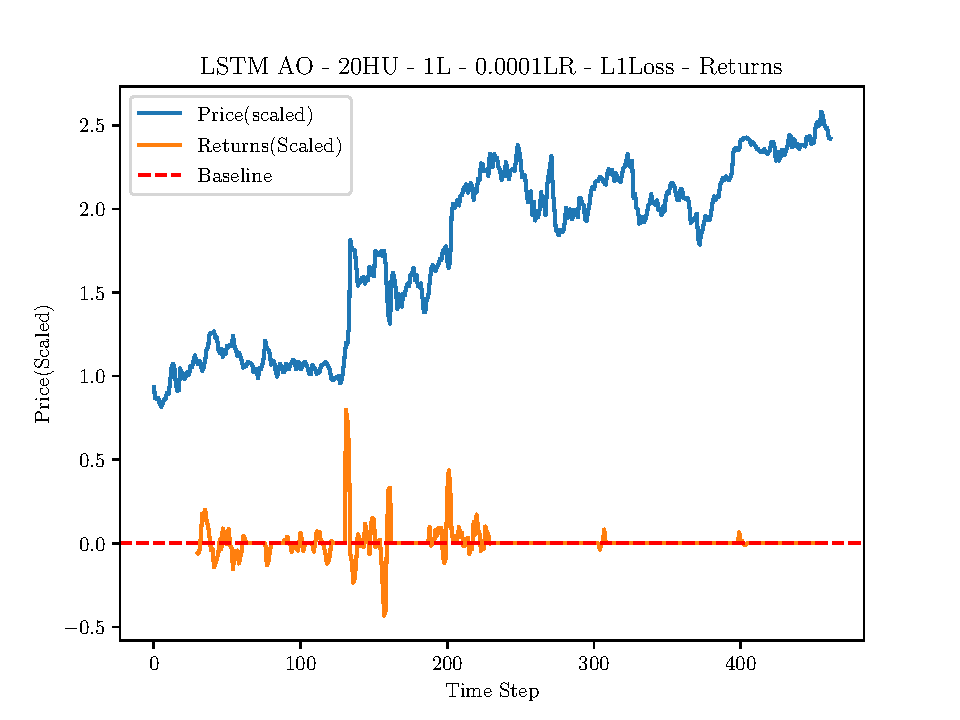
\includegraphics[width=0.5\textwidth, trim=20 0 20 10, clip]{plots/LSTM AO - 20HU - 1L - 0.0001LR - L1Loss-returns.pdf}
    \caption{Returns of the model with 20 hidden units and 1 layer. Although the model has the highest return, it does not handle stock prices that are much higher than the training data.}
    \label{fig:20HU_1L_returns}
\end{figure}

\begin{figure}[h]
    \centering
    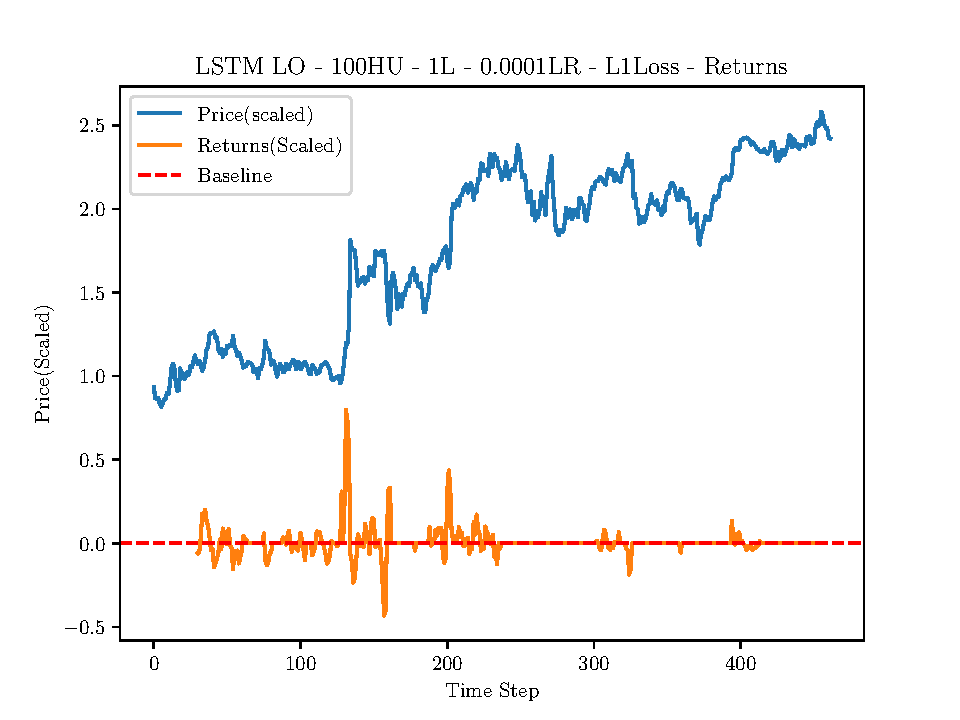
\includegraphics[width=0.5\textwidth, trim=20 0 20 10, clip]{plots/LSTM LO - 100HU - 1L - 0.0001LR - L1Loss-returns.pdf}
    \caption{Returns of the model with 20 hidden units and 1 layer. Does not perform as well as the 20 hidden unit model but does manage to make some successful trades at higher prices.}
    \label{fig:100HU_1L_returns}
\end{figure}

While the 20 hidden unit model did perform the best with the strategy, the loss was higher and upon inspection of the returns plot(Figure \ref{fig:20HU_1L_returns}), it can be seen that this model does not handle stock prices that are much higher than the training data. The 100 hidden unit models(Figure \ref{fig:100HU_1L_returns}) perform worse but do manage to make some successful trades at these higher prices. For this reason I am choosing the w/last 100HU 1L L1Loss model as the model to test on the test set.

\subsection{Final Test}

\begin{figure}[h]
    \centering
    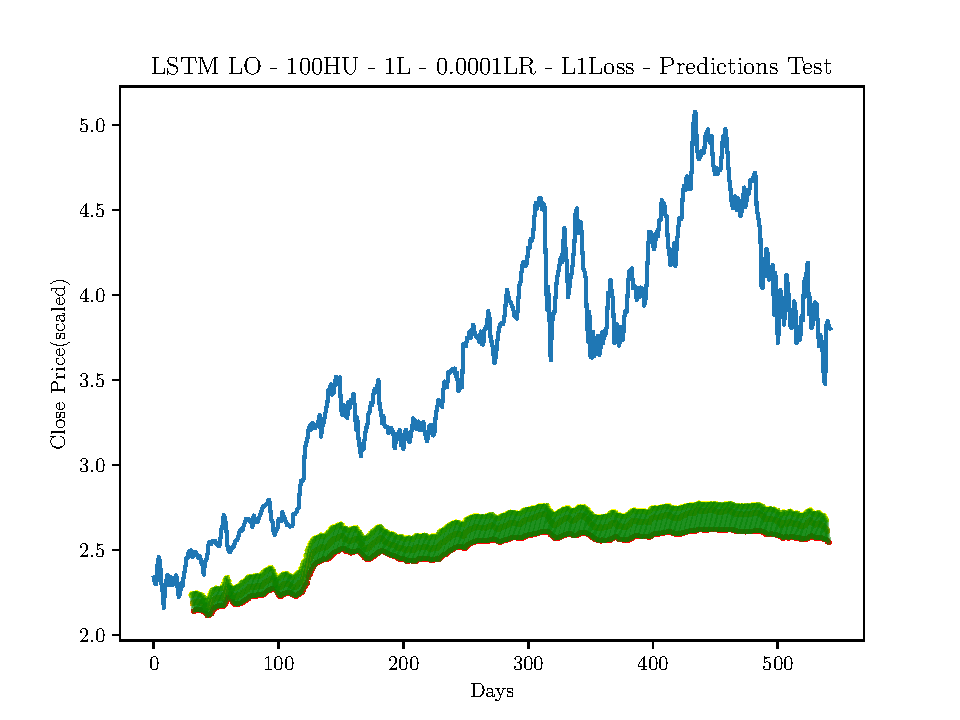
\includegraphics[width=0.5\textwidth, trim=20 0 20 10, clip]{plots/LSTM LO - 100HU - 1L - 0.0001LR - L1Loss-predictions-test.pdf}
    \caption{Predictions of the w/last 100HU 1L L1Loss model on the test set. Standardised prices in the test set are still too high relative to the training set for the model to be useful.}
    \label{fig:test_predtictions}
\end{figure}

The final test was conducted on the test set using the w/last 100HU 1L L1Loss model. Unfortunately, the model was a complete failure since the prices in the test set were much higher than the training set(Figure \ref{fig:test_predtictions}). Even though the dataset was standardised, the prices were so much higher(values of 4 - 5 after standardisation) that the model always predicted the price to decrease. After getting this result, I attempted to run the other models on the test set to see if any of them would work. Unfortunately, none of the models worked on the test set.


\section{Conclusion}

This assignment aimed to predict stock prices using an LSTM model to facilitate a simple but successful trading strategy. Unfortunately, the final model architecture, data preprocessing, and hyperparameters did not produce a model that could predict stock prices effectively. The model was heavily overfitting to the training data and could not generalise to the test set. The model was unable to handle stock prices that were much higher than the training data.

I think the main problem comes from the data preprocessing. The dataset was standardised using the z-score method, with the mean and standard deviation estimated from the training set and subsequently applied to the test set. Although this method is useful when inference inputs could be outside the range of the training set, it still does not handle the case where the values are much higher than the training set. I think a better strategy might be to use a smaller training set or normalise the data using a different method. 

Overfitting was another issue. Data augmentation could help here, either by adding noise to the data or by creating some synthetic data.

The strategy used was also very naive and did not take into account transaction costs, slippage, or other factors that would be present in a real-world scenario. A more sophisticated strategy could be used to improve the model's performance.




